\documentclass[../../../main.tex]{subfiles}
\begin{document}

%%%%%%%%%%%%%%%%%%%%%%%%%%%%%%%%%%%%%%%%%
%%%%%%%%%%%%%%%%%%%%%%%%%%%%%%%%%%%%%%%%%
%%%%%%%%%%%%%%%%%%%%%%%%%%%%%%%%%%%%%%%%%
\chapter{Area under curve}


An example of two gaussian curves:

\pgfmathdeclarefunction{gauss}{2}{%
  \pgfmathparse{1/(#2*sqrt(2*pi))*exp(-((x-#1)^2)/(2*#2^2))}%
}

\begin{center}
\begin{tikzpicture}
\begin{axis}[
  no markers, domain=0:10, samples=100,
  axis lines*=left, xlabel=$x$, ylabel=$y$,
  every axis y label/.style={at=(current axis.above origin),anchor=south},
  every axis x label/.style={at=(current axis.right of origin),anchor=west},
  height=5cm, width=12cm,
  xtick={4,6.5}, ytick=\empty,
  enlargelimits=false, clip=false, axis on top,
  grid = major
  ]
  \addplot [fill=cyan!20, draw=none, domain=0:5.96] {gauss(6.5,1)} \closedcycle;
  \addplot [very thick,cyan!50!black] {gauss(4,1)};
  \addplot [very thick,cyan!50!black] {gauss(6.5,1)};


\draw [yshift=-0.6cm, latex-latex](axis cs:4,0) -- node [fill=white] {$1.96\sigma$} (axis cs:5.96,0);
\end{axis}

\end{tikzpicture}
\end{center}

\noindent
Another example:

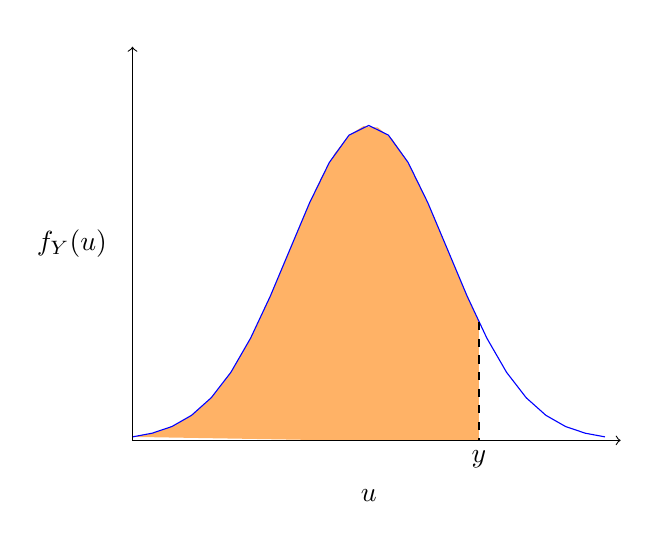
\begin{tikzpicture}
% define normal distribution function 'normaltwo'
    \def\normaltwo{\x,{4*1/exp(((\x-3)^2)/2)}}
 
% input y parameter
    \def\y{4.4}
 
% this line calculates f(y)
    \def\fy{4*1/exp(((\y-3)^2)/2)}
 
% Shade orange area underneath curve.
    \fill [fill=orange!60] (2.6,0) -- plot[domain=0:4.4] (\normaltwo) -- ({\y},0) -- cycle;
 
% Draw and label normal distribution function
    \draw[color=blue,domain=0:6] plot (\normaltwo) node[right] {};
 
% Add dashed line dropping down from normal.
    \draw[dashed] ({\y},{\fy}) -- ({\y},0) node[below] {$y$};
 
% Optional: Add axis labels
    \draw (-.2,2.5) node[left] {$f_Y(u)$};
    \draw (3,-.5) node[below] {$u$};
 
% Optional: Add axes
    \draw[->] (0,0) -- (6.2,0) node[right] {};
    \draw[->] (0,0) -- (0,5) node[above] {};
 
\end{tikzpicture}

\noindent
A very manually constructed curve:

\begin{center}
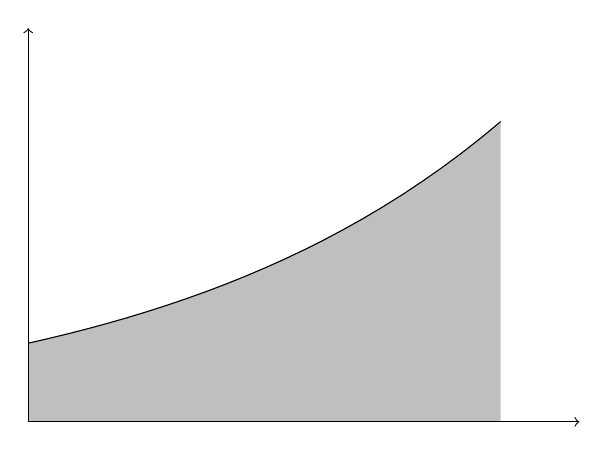
\begin{tikzpicture}

  \def\domMin{0}
  \def\domMax{6}
  \def\maxY{5}
  \def\maxX{7}

  % Define the function
  \def\expcurve2{\x,{1.25^\x}}
  \def\normaltwo{\x,{4*1/exp(((\x-3)^2)/2)}}
  
  % Fill the area under the line.
  \fill [fill=lightgray] (0, 0) -- plot[domain=\domMin:\domMax] (\expcurve2) -- (\domMax, 0) -- cycle;
  
  % Draw the line
  \draw[domain=\domMin:\domMax] plot (\expcurve2) {};

  
  % Axes
  \draw[->] (0, 0) -- (\maxX, 0);
  \draw[->] (0, 0) -- (0, \maxY);
  
\end{tikzpicture}
\end{center}

\noindent
A uniform distribution:

\begin{center}
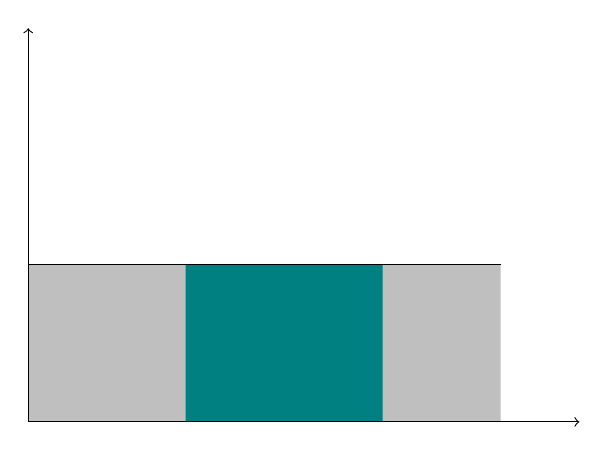
\begin{tikzpicture}

  \def\domMin{0}
  \def\domMax{6}
  \def\maxY{5}
  \def\maxX{7}

  % Define the function
  \def\dist{\x,{2}}

  % Fill the area under the line.
  \fill [fill=lightgray] (0, 0) -- plot[domain=\domMin:\domMax] (\dist) -- (\domMax, 0) -- cycle;

  % Fill a chunk.
  \fill [fill=teal] (2, 0) -- (2, 2) -- (4.5, 2) -- (4.5, 0) -- (2, 0);
  
  % Draw the line
  \draw[domain=\domMin:\domMax] plot (\dist) {};

  % Axes
  \draw[->] (0, 0) -- (\maxX, 0);
  \draw[->] (0, 0) -- (0, \maxY);
  
\end{tikzpicture}
\end{center}

\noindent
Simple somepin' or other:

\begin{center}
  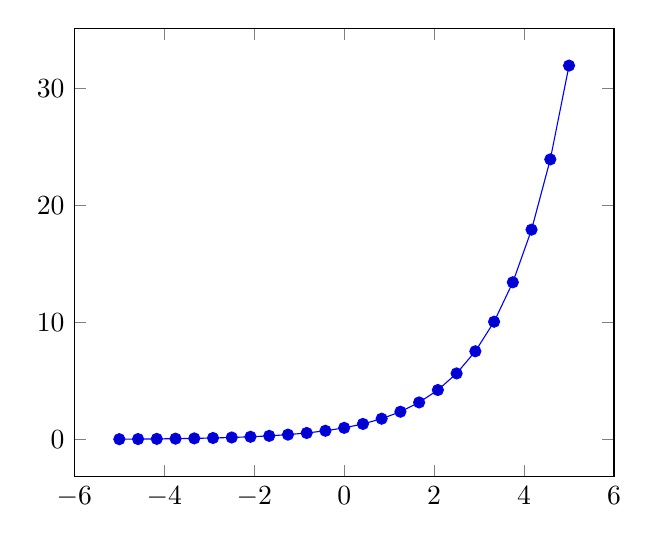
\begin{tikzpicture}
    \begin{axis}[]
      \addplot {2^x};
    \end{axis}
  \end{tikzpicture}
\end{center}

\noindent
Makin' it better:

\begin{center}
  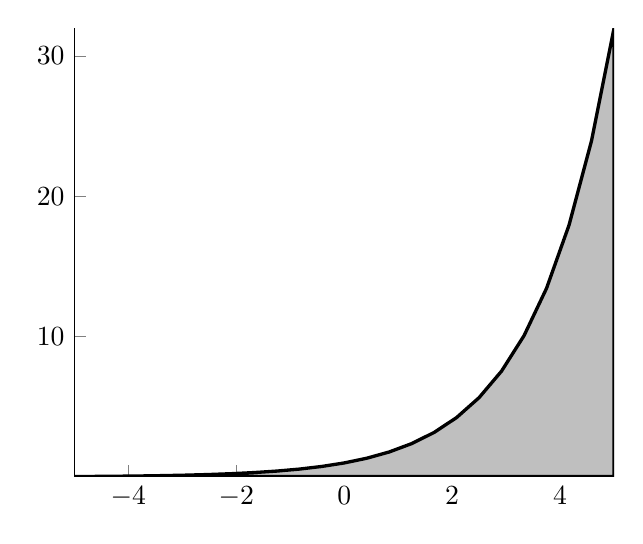
\begin{tikzpicture}
    \begin{axis}[
      no markers, % no dots
      axis lines*=left, % don't show axes on top and right
      enlargelimits=false % don't put space around the curve
      ]
      \addplot[fill=lightgray, very thick] {2^x} \closedcycle; % \closedcycle puts a line down the right side
    \end{axis}
  \end{tikzpicture}
\end{center}

\noindent
Specifying the coordinates:

\begin{center}
  \begin{tikzpicture}
    \begin{axis}[enlargelimits=false]
      \addplot coordinates{(1, 2) (2, 4) (3, 9) (4, 16) (5, 25)};
    \end{axis}
  \end{tikzpicture}
\end{center}

\noindent
Smooth curve:

\begin{center}
  \begin{tikzpicture}
    \begin{axis}[enlargelimits=false]
      \addplot[smooth] coordinates{(1, 2) (2, 4) (3, 9) (4, 16) (5, 25)};
    \end{axis}
  \end{tikzpicture}
\end{center}

\noindent
Filling it in:

\begin{center}
  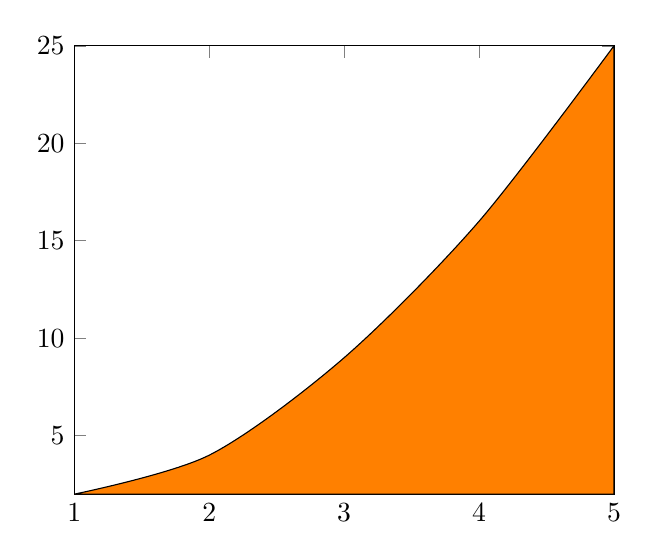
\begin{tikzpicture}
    \begin{axis}[enlargelimits=false]
      \addplot[smooth, fill=orange] coordinates{(1, 2) (2, 4) (3, 9) (4, 16) (5, 25)} \closedcycle;
    \end{axis}
  \end{tikzpicture}
\end{center}

\noindent
Adding points in:

\begin{center}
  \begin{tikzpicture}
    \begin{axis}[enlargelimits=false]
      \addplot[smooth, fill=orange] coordinates{(1, 2) (2, 4) (3, 9) (4, 16) (5, 25)} \closedcycle;
      \node[dot-point] at (axis cs:2, 4) [label=above:foo] {};
    \end{axis}
  \end{tikzpicture}
\end{center}

\noindent
Normal curve:

\begin{center}
  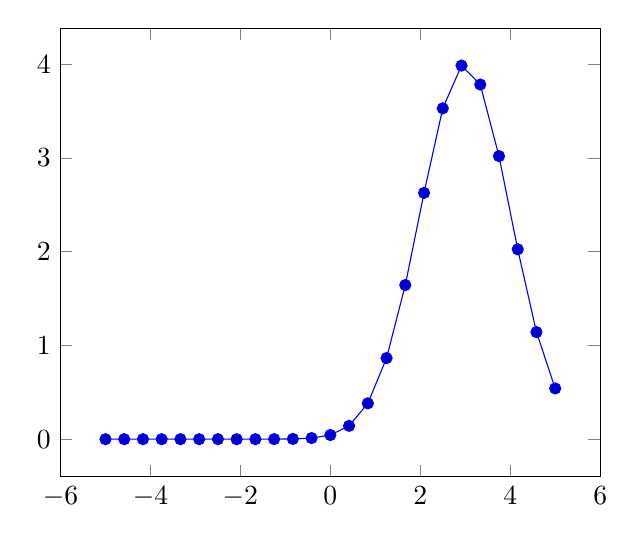
\begin{tikzpicture}
    \begin{axis}[]
      \addplot {4*1/exp(((x-3)^2)/2};
    \end{axis}
  \end{tikzpicture}
\end{center}

\noindent
Fix the domain:

\begin{center}
  \begin{tikzpicture}
    \begin{axis}[]
      \addplot[domain=0:6] {4*1/exp(((x-3)^2)/2};
    \end{axis}
  \end{tikzpicture}
\end{center}

\noindent
Make it better:

\begin{center}
  \begin{tikzpicture}
    \begin{axis}[
      no markers, % no dots
      axis lines*=left, % don't show axes on top and right
      enlargelimits=false % don't put space around the curve
      ]
      \addplot[domain=0:6, samples=41] {4*1/exp(((x-3)^2)/2};
    \end{axis}
  \end{tikzpicture}
\end{center}

\noindent
Fill in area under the curve:

\begin{center}
  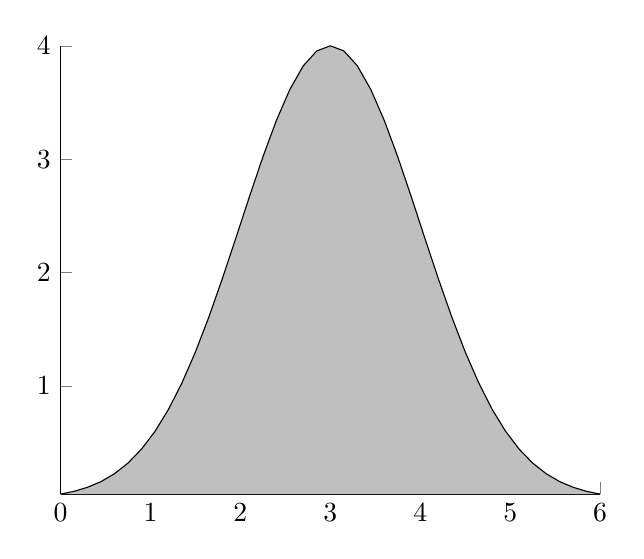
\begin{tikzpicture}
    \begin{axis}[
      no markers, % no dots
      axis lines*=left, % don't show axes on top and right
      enlargelimits=false % don't put space around the curve
      ]
      \addplot[domain=0:6, samples=41, fill=lightgray] {4*1/exp(((x-3)^2)/2};
    \end{axis}
  \end{tikzpicture}
\end{center}

\noindent
Draw some lines over the curve:

\begin{center}
  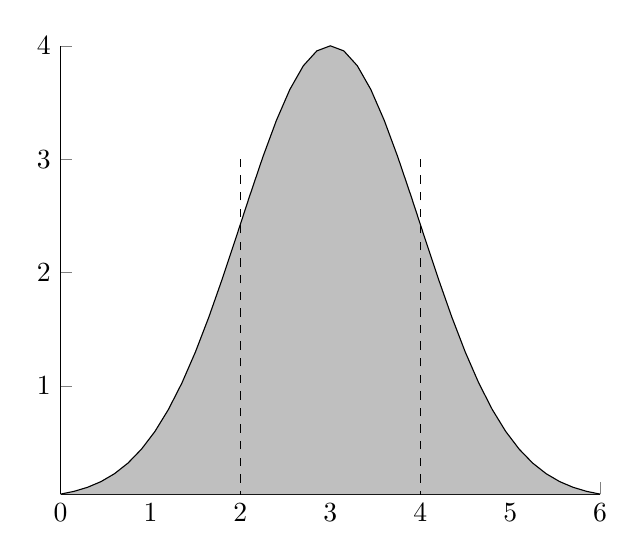
\begin{tikzpicture}
    \begin{axis}[
      no markers, % no dots
      axis lines*=left, % don't show axes on top and right
      enlargelimits=false % don't put space around the curve
      ]
      \addplot[domain=0:6, samples=41, fill=lightgray] {4*1/exp(((x-3)^2)/2};
      \draw[dashed] (2, 0) -- (2, 3);
      \draw[dashed] (4, 0) -- (4, 3);
    \end{axis}
  \end{tikzpicture}
\end{center}

\noindent
Shade an area under the curve:

\begin{center}
  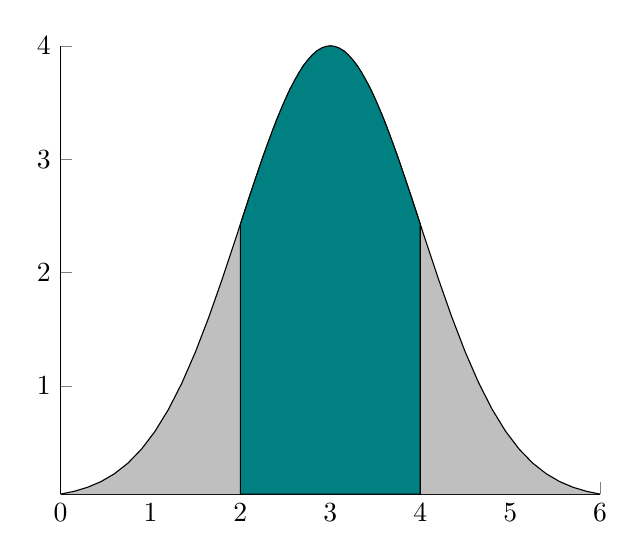
\begin{tikzpicture}
    \begin{axis}[
      no markers, % no dots
      axis lines*=left, % don't show axes on top and right
      enlargelimits=false % don't put space around the curve
      ]
      \addplot[domain=0:6, samples=41, fill=lightgray] {4*1/exp(((x-3)^2)/2};
      \addplot[domain=2:4, samples=41, fill=teal] {4*1/exp(((x-3)^2)/2} \closedcycle;
    \end{axis}
  \end{tikzpicture}
\end{center}

\noindent
Shade an area of a uniform distribution:

\begin{center}
  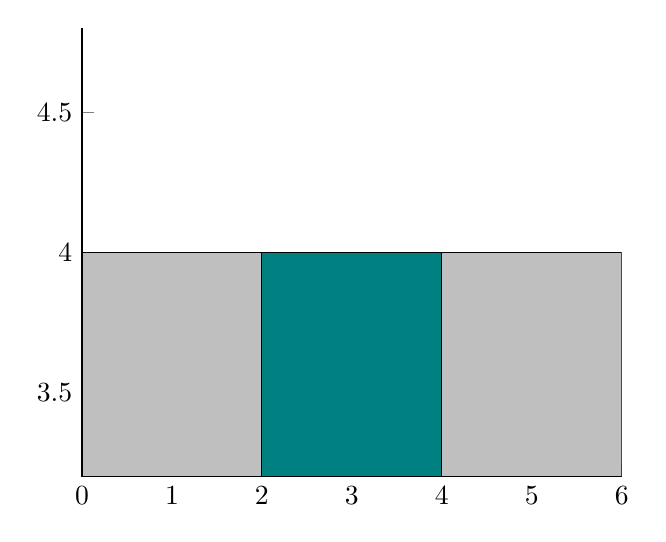
\begin{tikzpicture}
    \begin{axis}[
      no markers, % no dots
      axis lines*=left, % don't show axes on top and right
      enlargelimits=false % don't put space around the curve
      ]
      \addplot[domain=0:6, samples=41, fill=lightgray] {4} \closedcycle;
      \addplot[domain=2:4, samples=41, fill=teal] {4} \closedcycle;
    \end{axis}
  \end{tikzpicture}
\end{center}



\end{document}
